% latexmk -pvc -pdf
\documentclass[12pt, a4paper, openany]{book}
\usepackage[margin=2.5cm]{geometry}
\usepackage{titling}
\usepackage{titlesec}
\usepackage{amsmath,amsthm,amsfonts,amssymb}
\usepackage{dsfont}
\usepackage{mathtools}
\usepackage{braket}
\usepackage[font=scriptsize,labelfont=bf]{caption}
\usepackage[english]{babel}
\usepackage{float} 
\usepackage{pdflscape} 
\usepackage{cite}

\usepackage[T1]{fontenc}
\usepackage[utf8]{inputenc}

\usepackage{datetime}
\newdateformat{monthyeardate}{%
  \monthname[\THEMONTH], \THEYEAR}

\usepackage{graphicx}
\newenvironment{Figure}
    {\par\medskip\noindent\minipage{\linewidth}}
    {\endminipage\par\medskip}
\usepackage{tabularx}

\newenvironment{abstract}
{\clearpage \thispagestyle{empty} \null \vfill \begin{center} \bfseries \large Abstract \end{center}}
{\vfill \null \clearpage}

\newenvironment{impactstatement}
{\clearpage \thispagestyle{empty} \null \vfill \begin{center} \bfseries \large Impact Statement \end{center}}
{\vfill \null \clearpage}


% Colours:
\usepackage[table]{xcolor} % for setting colors
\definecolor{purple}{RGB}{117,77,226}

\usepackage[bookmarksopen,
  pagebackref,
  pdfpagelayout=TwoPageRight,
  colorlinks=true,
  urlcolor=purple,
  citecolor=purple,
  filecolor=purple,
  linkcolor=purple,
  ]
{hyperref}

\usepackage{listings}
\usepackage{xcolor} % Necessary to define custom colors

\definecolor{softblue}{rgb}{0.3, 0.5, 0.8}
\definecolor{darkergreen}{rgb}{0, 0.5, 0}

\lstset{
  basicstyle=\ttfamily\small, % Set the typeface to typewriter and small size
  breaklines=true, % Enable line breaking
  postbreak=\mbox{\textcolor{red}{$\hookrightarrow$}\space}, % Marker for line breaks
  numbers=left, % Line numbers on left
  numberstyle=\tiny, % Set the size of the numbers
}

\lstdefinestyle{mystyleC}{
    language=C,      
    commentstyle=\color{softblue},
    morecomment=[l]{//},  % Line comment
}

\lstdefinestyle{mystylePython}{
    language=Python,      
    commentstyle=\color{darkergreen},
    morecomment=[l]{//},  % Line comment
}

\titleformat{\chapter}[display]
  {\normalfont\bfseries}{}{0pt}{\Huge}


% Required packages
\usepackage{catchfile}

% Command to execute texcount and capture the word count
\newcommand\wordcount[1]{
    \immediate\write18{texcount #1.tex | grep "Words in text" | cut -d: -f2 > #1.wordcount.tmp}
    \CatchFileDef{\mywordcount}{#1.wordcount.tmp}{}
    \immediate\write18{rm #1.wordcount.tmp} % to remove the temporary file
    \mywordcount % to print the word count
}


\begin{document}

\begin{titlepage}
\begin{center}
    {\Huge BedSAT: Antarctica}\\ [1cm] 
    {\Large Exploring what lies beneath using big data and modelling}\\
    \vspace{5cm}
    {\large Ana Fabela Hinojosa\footnote{ana.fabelahinojosa1@monash.edu}}\\
    \monthyeardate\today\\ [1cm]
    Supervisors:\\
    Dr. Felicity McCormack\\
    Dr Jason Roberts\\
    Dr Richard Jones\\ [2cm]
    Panel:\\
    Dr. Fabio Capitanio \\
    Dr. Andrew Gunn \\
    Dr. Ariaan Purich \\ [3.5cm]
    \includegraphics[scale=0.2]{logos.png}

    \end{center}

\end{titlepage}


%----------------------------------------------------------------------------------------
%   QUOTATION PAGE
%----------------------------------------------------------------------------------------
% \vspace*{0.2\textheight}

% \noindent{``El alacrán clavándose el aguijón, harto de ser un alacrán pero necesitando de su alacranidad para acabar con el alacrán''.}\bigbreak
% % \vspace{-2cm}
% \hfill Julio Cortázar\bigbreak

\begin{impactstatement}\label{impactstatement}
Antarctica's bed topography data currently has uncertainties of hundreds of meters in elevation due to sparse and unevenly distributed radar surveys, significantly limiting our ability to predict ice sheet behavior and sea level rise contributions. Through the BedSAT project, we are developing a novel modelling approach that integrates remote sensing data and airborne derived estimates with mathematical and numerical ice flow models to substantially improve bed topography resolution and accuracy. We aim to derive a continent-wide bed topography dataset and conduct sensitivity analyses of dynamic ice loss to different realisations of topographic roughness through 2300.
Our work will quantify how bed topography uncertainties affect ice mass loss projections. This improved understanding can provide more reliable sea level rise predictions, and enable evidence-based policy decisions for climate adaptation strategies. Our open-source approach and FAIR data principles will ensure these improvements benefit the broader scientific community and support more effective climate change mitigation planning for vulnerable coastal communities.
\end{impactstatement}

% \chapter*{Acknowledgements}

\tableofcontents

% introduction
\chapter{Antarctica's Landscape}\label{why}
\section{Climate Impacts and Global Significance}

The polar regions are losing ice, and their oceans are changing rapidly\cite{O_C_in_changingClimate}. The consequences of this extend to the whole planet and it is crucial for us to understand them to be able to evaluate the costs and benefits of potential mitigation. 

Changes in different kinds of polar ice affect many connected systems. Of particular concern is the accelerating loss of continental ice sheets (glacial ice masses on land) in both Greenland and Antarctica, which has become a major contributor to global sea level rise\cite{O_C_in_changingClimate}. Impacts extend beyond direct ice loss: As fresh water from melting ice sheets is added into the ocean, it increases ocean stratification disrupting global thermohaline circulation\cite{Jacobs_2004}. In addition, cold freshwater can dissolve larger amounts of $\mathrm{CO_2}$ than regular ocean water creating corrosive conditions\cite{O_C_in_changingClimate}.
 
While there is high confidence in current ice loss and retreat observations in many areas, there is more uncertainty about the mechanisms driving these changes and their future progression\cite{Fox-Kemper_2021}. Uncertainty increases in regions with variable bed conditions, where characteristics like ``slipperiness'' and ``roughness'' are difficult to verify via direct samples. Other problematic areas involve the ice sheet's grounding line (GL). The retreat rate depends crucially on topographical features like pinning points, as these are locations where the GL is most stable and ice-sheet retreat will slow\cite{Fox-Kemper_2021}. However, major knowledge gaps persist in mapping bed topography across Antarctic ice sheet margins - with over half of all margin areas having insufficient data within 5 km of the grounding zone\cite{RINGS_2022}. Addressing this data gap through systematic mapping efforts would significantly improve both our understanding of current ice dynamics and the accuracy of ice-sheet models projecting future changes.

\chapter{Topography of Antarctica}\label{review}

Bed topography is one of the most crucial boundary conditions that influences ice flow and loss from the Antarctic Ice Sheet (AIS)\cite{Morlighem_2020}. Bed topography datasets are typically generated from airborne radar surveys, which are sparse and unevenly distributed across the Antarctic continent (see figure \ref{fig:BedMAP}). Interpolation schemes to ``gap fill'' these sparse datasets yield bed topography estimates that have high uncertainties (i.e. multiple hundreds of metres in elevation uncertainty; Morlighem et al., 2020) which propagate in simulations of AIS evolution under climate change\cite{Castleman_2022}. Given the logistical challenges of accessing large parts of the Antarctic continent, there is a crucial need for alternative approaches, that integrate diverse and possibly more spatially complete data streams – including satellite data.
\begin{figure}[H] % Forces the figure exactly HERE
    \includegraphics[scale=0.4]{bedmap.png}
    \caption{Distribution of BedMAP\{1,2,3\} data tracks (Source: bedmap.scar.org).}
    \label{fig:BedMAP}
\end{figure}

\section{Approaches to Bed Topography Reconstruction}

Obtaining information about the conditions at the base of the ice-sheet often relies on indirect modelling methods that operate in two fundamentally different directions:
\begin{itemize}
    \item\textbf{Forward models}
    From bed topography data, simulate ice flow to predict surface conditions. They use known or assumed basal properties to model how the ice sheet will respond.
    
    \begin{itemize}
           \item\textbf{4dvar}: Four-dimensional variational data assimilation - Minimizes the difference between model predictions and observations across a time window. Mainly used to optimize model parameters and initial conditions\cite{Morlighem_Goldberg_2024}. Can handle time-varying data and evolving glacier states, making it more suitable for dynamic systems unlike control methods, this makes them more computationally demanding\cite{Morlighem_Goldberg_2024}.

            \item\textbf{Geostatistics} Statistical methods specialized for analyzing spatially correlated data. In glaciology, this approach is used to interpolate between sparse measurements and characterise spatial patterns in bed properties, often employing techniques like kriging\cite{Mackie_2020}.

            \item\textbf{EnKF} Ensemble Kalman Filter. A sequential data assimilation method that uses an ensemble of model states to estimate uncertainty and update model parameters based on observations\cite{Morlighem_Goldberg_2024}.
    \end{itemize}

    \item\textbf{Inversion models}
    Retrieval (or update) of bed topography and basal slipperiness from surface topography and velocity measurements\cite{deRydt_2013}.

        \begin{itemize}
            \item\textbf{Control method inversion}: A variational approach that minimizes mismatches between observed and simulated fields through a cost function approach. Remote sensing data and theoretical ice flow models are used to obtain basal conditions\cite{deRydt_2013}. Often needs regularization terms to prevent non-physical features or over-fitting\cite{Morlighem_Goldberg_2024}.

            \item\textbf{Mass conservation}: Used to constrain inversion models and fill data gaps by employing physical conservation laws, particularly effective for reconstructing bed topography where direct measurements are sparse~\cite{Morlighem_2017, Morlighem_2020}. Requires (contemporary) measurements of ice thickness at the inflow boundary to properly constrain the system\cite{Morlighem_Goldberg_2024}.

            \item\textbf{Markov Chain Monte Carlo (MCMC)}: A probabilistic method that generates sample distributions to quantify uncertainties in ice sheet parameters and models\cite{Morlighem_Goldberg_2024}. While powerful for uncertainty quantification, these methods remain computationally intensive for continental-scale ice sheet models\cite{Morlighem_Goldberg_2024}.
        \end{itemize}
    
\end{itemize} 
While each method has its strengths and limitations, the choice of approach often depends on the specific research objectives, data availability, and computational resources. Control methods and mass conservation approaches are widely used for steady-state reconstructions, while 4dvar and EnKF methods are better suited for time-evolving systems. Recent advances in computational power have made probabilistic methods like MCMC more feasible, offering valuable insights into parameter uncertainties.

\newpage
\section{Theoretical Frameworks}
These modeling approaches, particularly forward models, rely on theoretical frameworks that describe the relationship between bed topography and surface features. Many authors have explored this relationship to understand how basal conditions influence the ice surface profile features. Understanding how bed features manifest in surface observations requires a theoretical framework that connects these two domains. A pioneering contribution to this field was made by Budd \cite{Budd_1970}, who developed a model relating ice flow over bedrock perturbations to surface expressions using a two-dimensional biharmonic stress equation. 

The model's foundation rests on two key simplifications:
\begin{itemize}
    \item Most shear deformation occurs at the base of the ice sheet
    \item Explicit consideration of longitudinal stresses and strain-rates
\end{itemize}

The modelling carried out in\cite{Budd_1970} determined ice-sliding velocities for wide ranges of roughness, normal stress, and shear stress relevant to real glaciers\cite{Budd_1970}. Despite its robustness, Budd's mathematical framework remains notably underutilized in modern ice sheet modeling. This gap in application is particularly striking given today's advanced computational capabilities and high-resolution satellite observations. 
This begs the questions: What specific computational or theoretical advances are required to effectively integrate Budd's mathematical framework with contemporary high-resolution satellite observations? And once we integrate this model into modern ice sheet modelling, 
how does the accuracy of Budd's model compare to more complex modern approaches when predicting surface expressions from known bed topography features across different ice flow regimes?

\section{Modern Inversion Methods}\label{Ockenden_2022}

The shape and mechanical properties of the ice bed significantly influence how ice flows, with changes at the bed potentially leading to large differences in predicted ice loss rates\cite{Ockenden_2022}. Recent work by Ockenden et al. demonstrates both the capabilities and limitations of current inversion approaches in addressing this problem.

The core principle of the method by Ockenden et al. (2022) relies on the fact that variations in basal topography, slipperiness, and roughness cause measurable disturbances to the surface flow of the ice. Through linear perturbation analysis, they establish a systematic relationship between surface observations and bed conditions. This relationship can be expressed as $y=f(x)$, where $y$ represents surface measurements (velocity and topography), $x$ represents bed properties (topography and slipperiness), and $f$ is the forward model\cite{Gudmundsson_2008}. The inversion process, $x=f^{-1}(y)$, estimates bed conditions from surface observations.

The method works best when analyzing perturbations that are small relative to mean properties, under specific conditions including:
\begin{enumerate}
    \item A linear viscous medium ($n=1$)
    \item Non-linear sliding law ($m>0$)
    \item Steady-state conditions
    \item Spatially constant zero-order solutions
\end{enumerate}

Using high-resolution datasets (REMA surface elevation at 8m resolution and NASA ITS\_LIVE velocity at 120m resolution), their approach performs well for:
\begin{itemize}
    \item Areas with moderate topographic gradients
    \item Features not aligned with ice flow direction
    \item Medium-wavelength (5-50km) bedrock features
\end{itemize}

However, significant limitations emerge when:
\begin{itemize}
    \item Dealing with steep topography where the shallow-ice-stream approximation breaks down
    \item Handling variable slipperiness parameters
    \item Attempting to validate slipperiness predictions due to lack of ground-truth data
\end{itemize}

While modern satellite technology has revolutionized our understanding of ice sheets by providing unprecedented detail of surface features, these limitations highlight a key challenge in glaciology: we have yet to fully leverage this wealth of information to improve bed topography estimates in regions where radar data is sparse. This gap between rich surface datasets in certain regions and limited subglacial understanding motivates this investigation. It is of particular interest to us to develop the integration of more comprehensive models and modern computational capabilities.


\section{Current Opportunities}

We have highlighted above several persistent challenges in Antarctic bed topography reconstruction, and I have also included a description of current approaches. The works I chose to exemplify here, while theoretically robust, faces practical limitations. The inversion method employed by Ockenden et al. provides valuable insights but is limited by assumptions that do not capture the full complexity of ice-bed interactions, particularly when dealing with steep topography where the shallow-ice-stream approximation breaks down. Similarly, the sliding theory developed by Budd offers important physical insight but remains underutilized in modern ice sheet modeling despite today's advanced computational capabilities and high-resolution satellite observations.

A key question in this work is how surface features relate to ice thickness. Our current models struggle to capture the complex relationships created by basal roughness and variable friction zones. Additionally, we lack crucial data like basal friction measurements for accurate reconstruction. These challenges mean the results depend heavily on the assumptions built into models. Another key factor involves the dynamics at ice sheet margins. As noted by Nias (2018) in \cite{Nias_2018}, ``subtle variation in the geometry near the grounding line can trigger a response in the ice sheet that is felt hundreds of kilometers upstream.''
I want to understand how do changes in bed conditions and topographical features like ``slipperiness'',``roughness" and pinning points specifically influence the rate of grounding line retreat in continental ice sheets? This question is essential for accurate bed topography reconstruction and subsequent ice sheet evolution modeling. Similarly, ice viscosity is a critical factor since high viscosity ice near the surface tends to dampen bed topography signals significantly\cite{deRydt_2013}, creating potential misinterpretations of surface expressions. 

With BedSAT, I aim to build upon the theoretical foundations established by Budd and recent inversion methods. Our approach will help bridge the disconnect between surface observations and bed topography by utilizing a more realistic set of rheological and geometric assumptions.  This addresses another fundamental question in our field: To what extent do interpolation uncertainties in bed topography datasets affect the accuracy of Antarctic Ice Sheet evolution simulations under different climate change scenarios?

In addition, I plan to implement the methods in an iterative way, allowing us to improve results via an inversion-forward modelling validation cycle: The initially inverted bed topography will be used in the ice dynamics (forward) model with BedSAT's improved rheological and geometric assumptions, to then compare the resulting surface predictions with products like NASA'S ITS\_LIVE (see Chapter \ref{resources}). Part of my plan involves a systematization of this process via Machine learning methods. This will ultimately enhance the analyses in the final phase of my project.
 
% \wordcount{literature_review} words in this section.
% planning
\chapter{Methods}
\section{Aims}
 My research plan is structured around these three broad research questions:
\begin{enumerate}

    \item How does the bed topography manifest on the ice surface?

    \item To what extent do interpolation uncertainties in bed topography datasets affect the accuracy of Antarctic Ice Sheet evolution simulations under different climate change scenarios?

    \item What is the impact of variable bed conditions and topography on the rate of grounding line (GL) retreat in continental ice sheets?

\end{enumerate}

Underpinning these research questions are the following objectives (O):
\begin{itemize}
    \item{O1:} Develop an ice sheet modelling approach to assimilate satellite remote sensing datasets to improve knowledge of the bed (BedSAT) informed by mathematical models of ice flow over topography;

    \item{O2:} Derive a new bed topography for Antarctica using BedSAT;

    \item{O3:} Evaluate the impact of the improved bed topography on projections of ice mass loss from Antarctica under climate warming through sensitivity analyses. 
\end{itemize}

\section{Research plan methodology}

In order to achieve these objectives, each will be addressed in sequential phases. My primary focus is currently on O1: Deriving the BedSAT method. As the initial phase of O1, I am working on an investigation on the influence of different combinations of rheological and sliding law assumptions in ice sheet modeling. The goal of this investigation is to systematically understand the forward problem (how the bed affects the surface under different physical rules), and then use that knowledge to build a better inverse model (BedSAT). This foundational study will be the basis for my first peer-reviewed paper.

\subsection{Foundational Analysis of Bed-to-Surface Signal Transfer}\label{paper1}

The first critical step is to systematically quantify how fundamental physical assumptions influence the expression of subglacial topography at the ice surface.
This directly addresses my first research question: "How does the bed topography manifest on the ice surface?". This work will leverage the Ice-sheet and Sea-level System Model (ISSM) with a custom-built computational framework based on a synthetic bed topography database. See Chapter~\ref{progress} for detailed information. This systematic study will verify and validate the necessary set of constraints on bed-to-surface transfer functions that account for realistic ice dynamics. This comprehensive analysis will form the basis of the the first peer-reviewed manuscript of this PhD.

\subsection{Development of the BedSAT Inversion Framework}

By understanding how rheology and sliding conditions alter the surface expression of the bed, I can develop more physically robust transfer functions for the inversion process. The inversion model will be developed and tested using a regional catchment in Antarctica with extensive radar data, such as the Aurora Subglacial Basin (this data can be found in works such as~\cite{Young_2011}). The model will be constrained by available observations of surface velocity, thermal distribution, and ice thickness, this will allow for direct validation of the inversion results against known bed configurations. Furthermore, the robustness of the model will be ensured through grid independence testing and a sensitivity analysis of model assumptions.

\subsection{Derive a new bed topography for Antarctica using BedSAT}

I will apply the validated BedSAT methodology from O1 to the entire Antarctic continent, deriving a new continent-wide bed topography dataset. Using covariance properties from existing radar surveys, I will generate multiple realisations of the bed, each with unique and statistically-consistent topographic roughness.

\subsection{Evaluate the impact of the improved bed topography}

The new bed topography datasets will be used to conduct a sensitivity analysis of ice sheet model projections to 2300 CE. This will investigate the impact of the improved topography and different roughness realisations on ice dynamics, subglacial hydrology, and overall ice mass loss from Antarctica, directly addressing the project's main research questions.
\\
\textit{Note: Detailed methodological outlines for O2 and O3 will be developed following the completion and refinement of the BedSAT method in O1.}



% \wordcount{methodology} words in this section.
\chapter{Resources}

The project will require high performance computing resources (including compute and storage) from the National Computing Infrastructure (NCI). We anticipate requiring $\sim$250~k Service Units (SU) each quarter, and up to 500 TB of storage. These resources are already available via a Flagship between NCI and the Monash-led Australian Research Council project Securing Antarctica’s Environmental Future (SAEF).

\section*{Data management and archiving}

Data will be published adhering to FAIR principles (Findable, Accessible, Interoperable, Reusable), ensuring transparency and accessibility. The final bed topography datasets will be published at the Australian Antarctic Data Centre (AADC) under an open source licence. All production model outputs will be published with unique DOIs at repositories aligned with the corresponding journal articles. Model outputs – including production and other outputs – will be archived to tape at NCI using existing SAEF resources, as well as backed up to storage available through Monash MASSIVE M3 account aligned with project supervisor Dr McCormack. All journal articles published through this project will be open source, and tier 1 journals will be targeted.

\section*{Risk}

The project is highly feasible and low risk, given that it is a desk-based modelling and data assimilation project. All the data to be used in this project are freely available for download, and project supervisors are experts in ice sheet modelling using ISSM.

\textit{Fieldwork}\\
Fieldwork is not necessary to achieve the objectives of the project; however, there may be the opportunity to participate in fieldwork through the ICECAP airborne geophysics project (led CI of ICECAP is project supervisor Dr Jason Roberts, Australian Antarctic Division), which will be instrumental in training of geophysical instruments and in developing broader expertise in the field. \\


\section*{Career Development}

\textit{Conferences}\\
At least one conference will be attended each year. An international conference relevant to the discipline, e.g. the European Geophysical Union General Assembly, will be attended in the final year of the project.
\wordcount{resources} words in this section.
\chapter{Progress}\label{progress}
\section{Rheology and Sliding Study}\label{study1}
Building upon the diagnostic ISMIP-HOM experiments in~\cite{Pattyn_2008}, I extend the prognostic experiment F to systematically investigate the combined effects of rheology and basal sliding within this benchmark ice sheet model. The original experiment F included two scenarios: One with a frozen bed (no-slip) and another with linear sliding.
My study expands upon these conditions by also incorporating non-linear rheology. This addition generates four distinct scenarios for comparison:
\begin{compactitem}
    \item{\bf{S1}:} No-slip (frozen) bed + Linear rheology ($n=1$).
    \item{\bf{S2}:} No-slip (frozen) bed + Non-linear rheology ($n=4$).
    \item{\bf{S3}:} Linear sliding + Linear rheology ($n=1$).
    \item{\bf{S4}:} Linear sliding + Non-linear rheology ($n=4$).
\end{compactitem}
To utilise non-linear rheology and still have consistent simulations, I ensure that different model rheologies start from identical initial conditions. The method I follow is based on the re-scaling method by Getraer and Morlighem (2025)~\cite{Getraer_2025}. Their formula ensures that the initial ice viscosity—and therefore strain rates for a given stress—is identical between simulations with different rheologies.
The fundamental model for the deformation of glacial ice and the equations which govern ice flow is Glen's flow law. 
\begin{equation}
\mathbf{\dot{\varepsilon}} \,=\, A_{n}\,\mathbf{\tau}^{n},
\end{equation}
here the $\mathbf{\dot{\varepsilon}}$ is the strain rate, $A_n$ is the rate factor and $\mathbf{\tau}^{n}$ is the stress deviator.
For the non-linear scenarios I am considering $n = 4$, since the assumption of $n = 3$ for ice deformation is not universally supported and values of $n > 3$ have been inferred from real‐world glaciers.
\begin{figure}[H]
    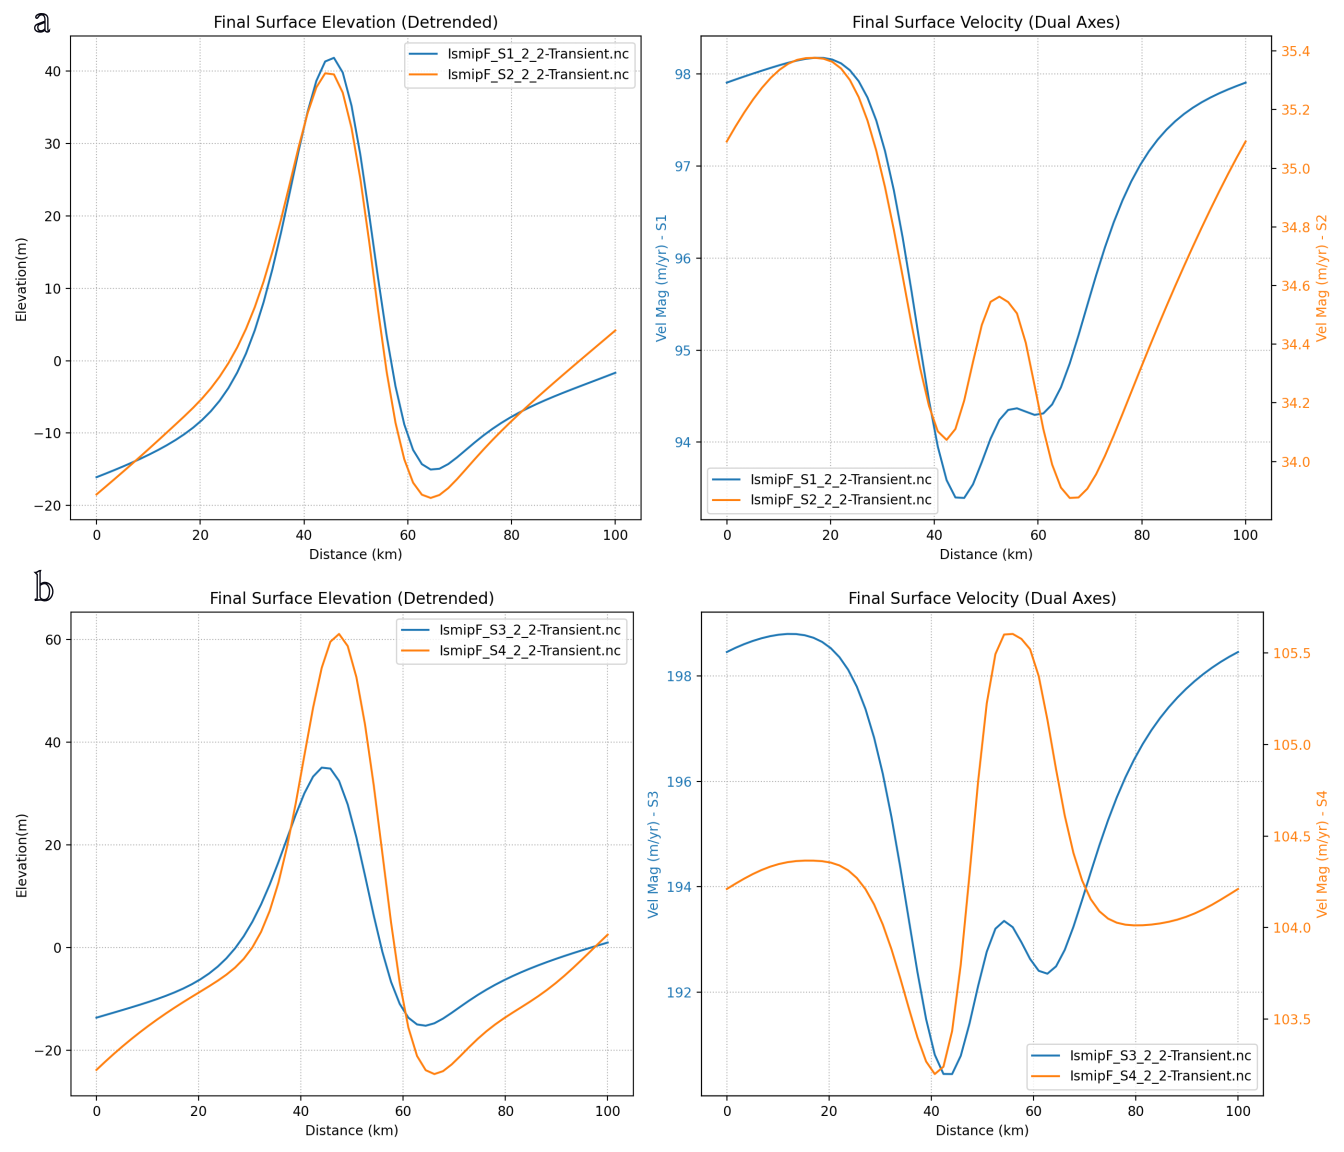
\includegraphics[scale=0.40]{figures/combined_elevation_detrended_surface_velocity_['S1']_['S2']_['S3']_['S4'].png}
    \caption{(a) Final surface elevations and velocities for the original frozen bed Experiment F (S1: linear rheology) and the corresponding transformed to non-linear rheology experiment (S2) (b) Final surface elevations and velocities for the original sliding bed Experiment F (S3: linear rheology) and the corresponding transformed to non-linear rheology experiment (S4).}
    \label{fig:elev_vel_S1_S2_S3_S4}
\end{figure}
The linear results depicted in blue in Figure~\ref{fig:elev_vel_S1_S2_S3_S4} are consistent with the surface elevation and velocities found for Experiment F in~\cite{Pattyn_2008}. Meanwhile, the non-linear scenarios (S2 and S4) shown in orange  represent the first key finding of this analysis. The marked differences in both final surface elevation and velocity compared to the linear counterparts (S1, S3) provide crucial evidence for my first research question (``How does the bed topography manifest on the ice surface?''). Using $n = 4$ leads to a strong non-linear relationship where a small increase in stress yields a much larger increase in deformation. The results utilise an optimised grid meshing and demonstrate that the choice of rheology is an important control on the bed-to-surface signal transfer, implying that a succesful inversion framework like BedSAT must account for non-linear effects.
\newpage
\section{Data Processing, Visualisation and Analysis Tools}\label{analysis_tools}
The core of this study is a time evolution flow simulation of fully grounded ice over 300 years with daily time steps. This simulation is designed to systematically investigate the relationship between basal geometry, ice rheology and flow response by running a series of ISMIP-HOM style experiments~\cite{Pattyn_2008} that can later be analysed in detail with other data processing tools.
\begin{figure}[H]
    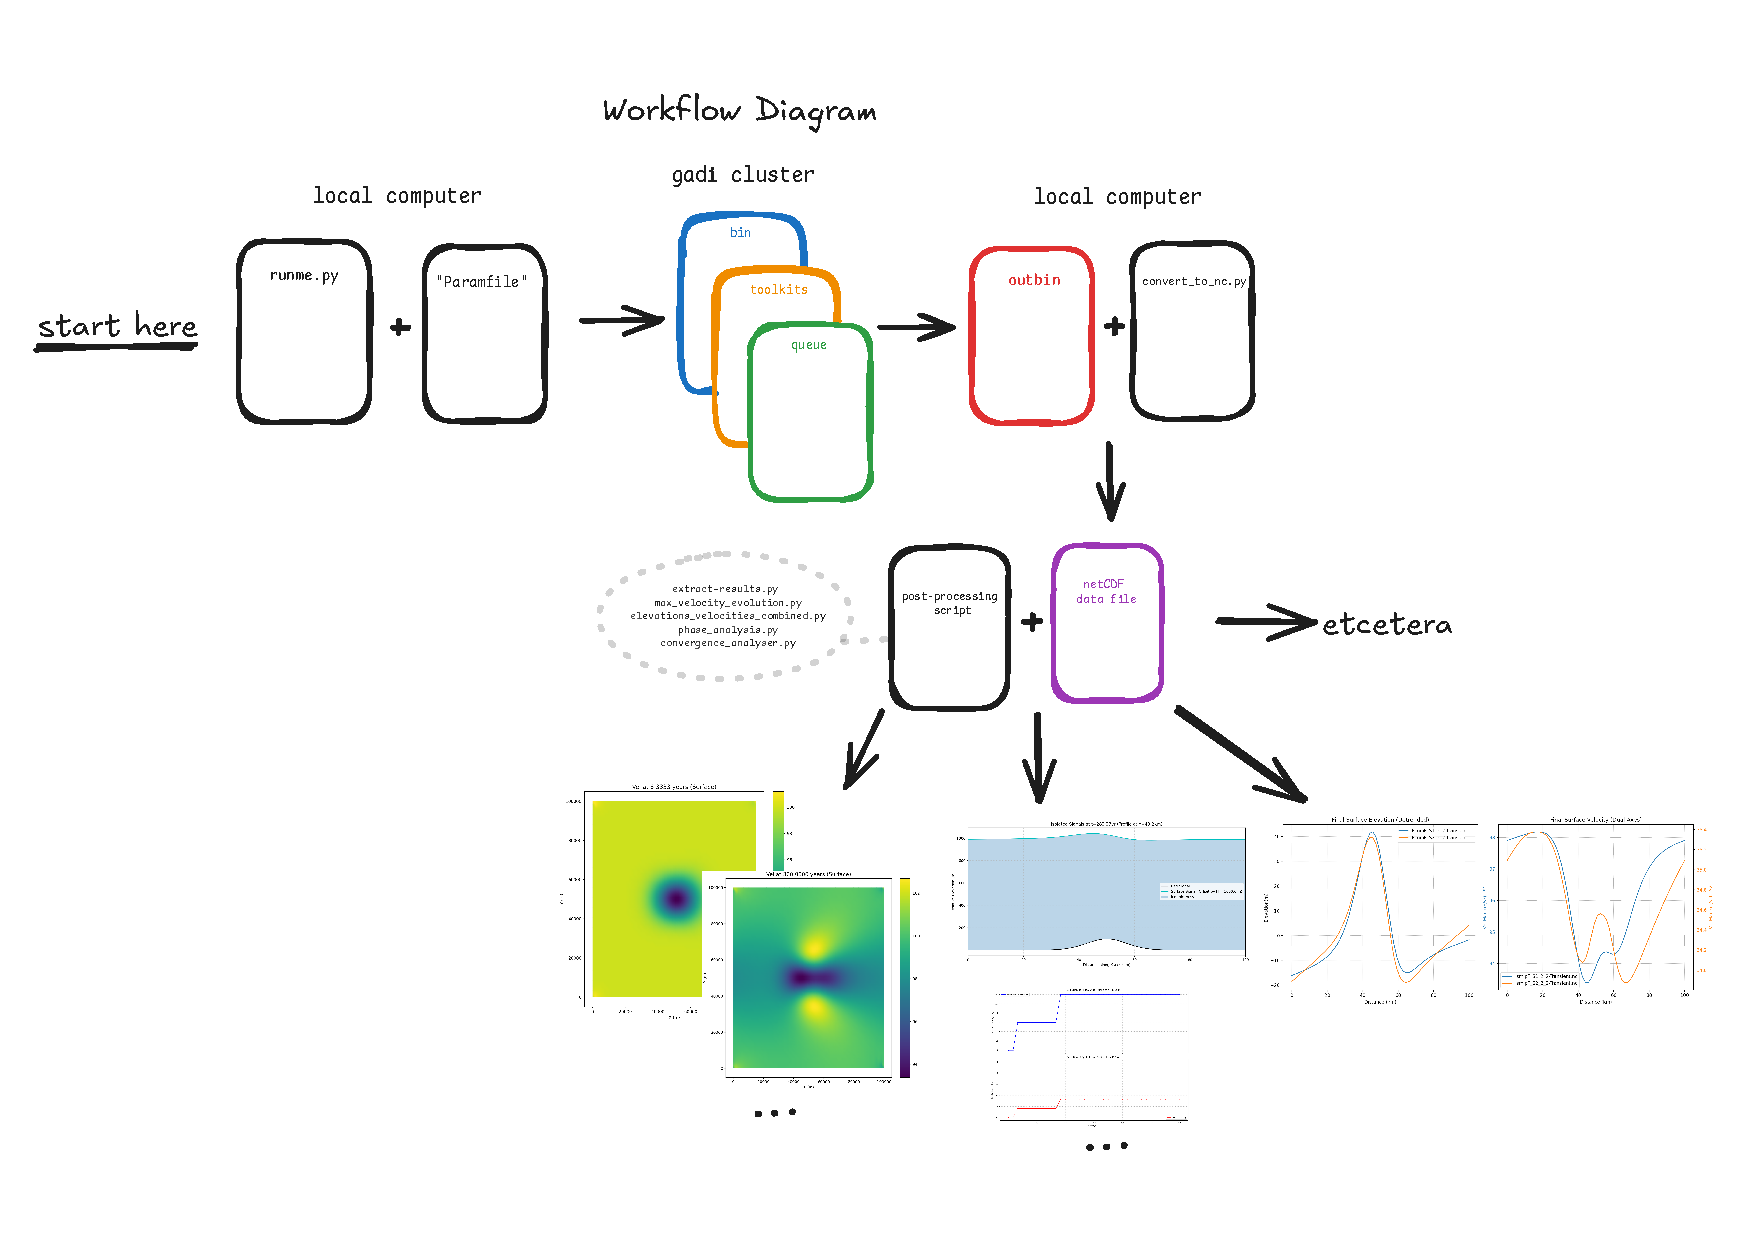
\includegraphics[scale=0.55]{figures/workflow_diagram.pdf}
    \caption{Diagrammatic representation of the current workflow using my ice simulation and analysis suite.}
    \label{fig:workflow}
\end{figure}
The scripts I've developed include a binary file to into NetCDF converter, a transient simulation analyser that generate visualisations of key fields like velocity and pressure. and other additional scripts that create specific scientific analysis and plots.
\subsection{Grid Independence}\label{grid_ind}
Grid optimisation testing involved simulations with 16 distinct mesh resolutions, varying both the horizontal (H) and vertical (V) grid densities independently. The resolution scaling factors tested are $2.0$ i.e. double the resolution, $0.5$ i.e. half the mesh resolution, $1.0$ i.e. no scaling and $1.5$ i.e. 50\% scaling. I designated the solution from the highest resolution mesh, corresponding to scaling factors of ($H=2.0, V=2.0$) as the reference solution. Refined meshes (either horizontal or vertical) often require smaller time steps to satisfy the Courant-Friedrichs-Lewy (CFL) condition and maintain solver stability. To satisfy this criterion I scaled the time step for each simulation matching the largest resolution factor independently if it was horizontal or vertical scaling.
\begin{figure}[H]
    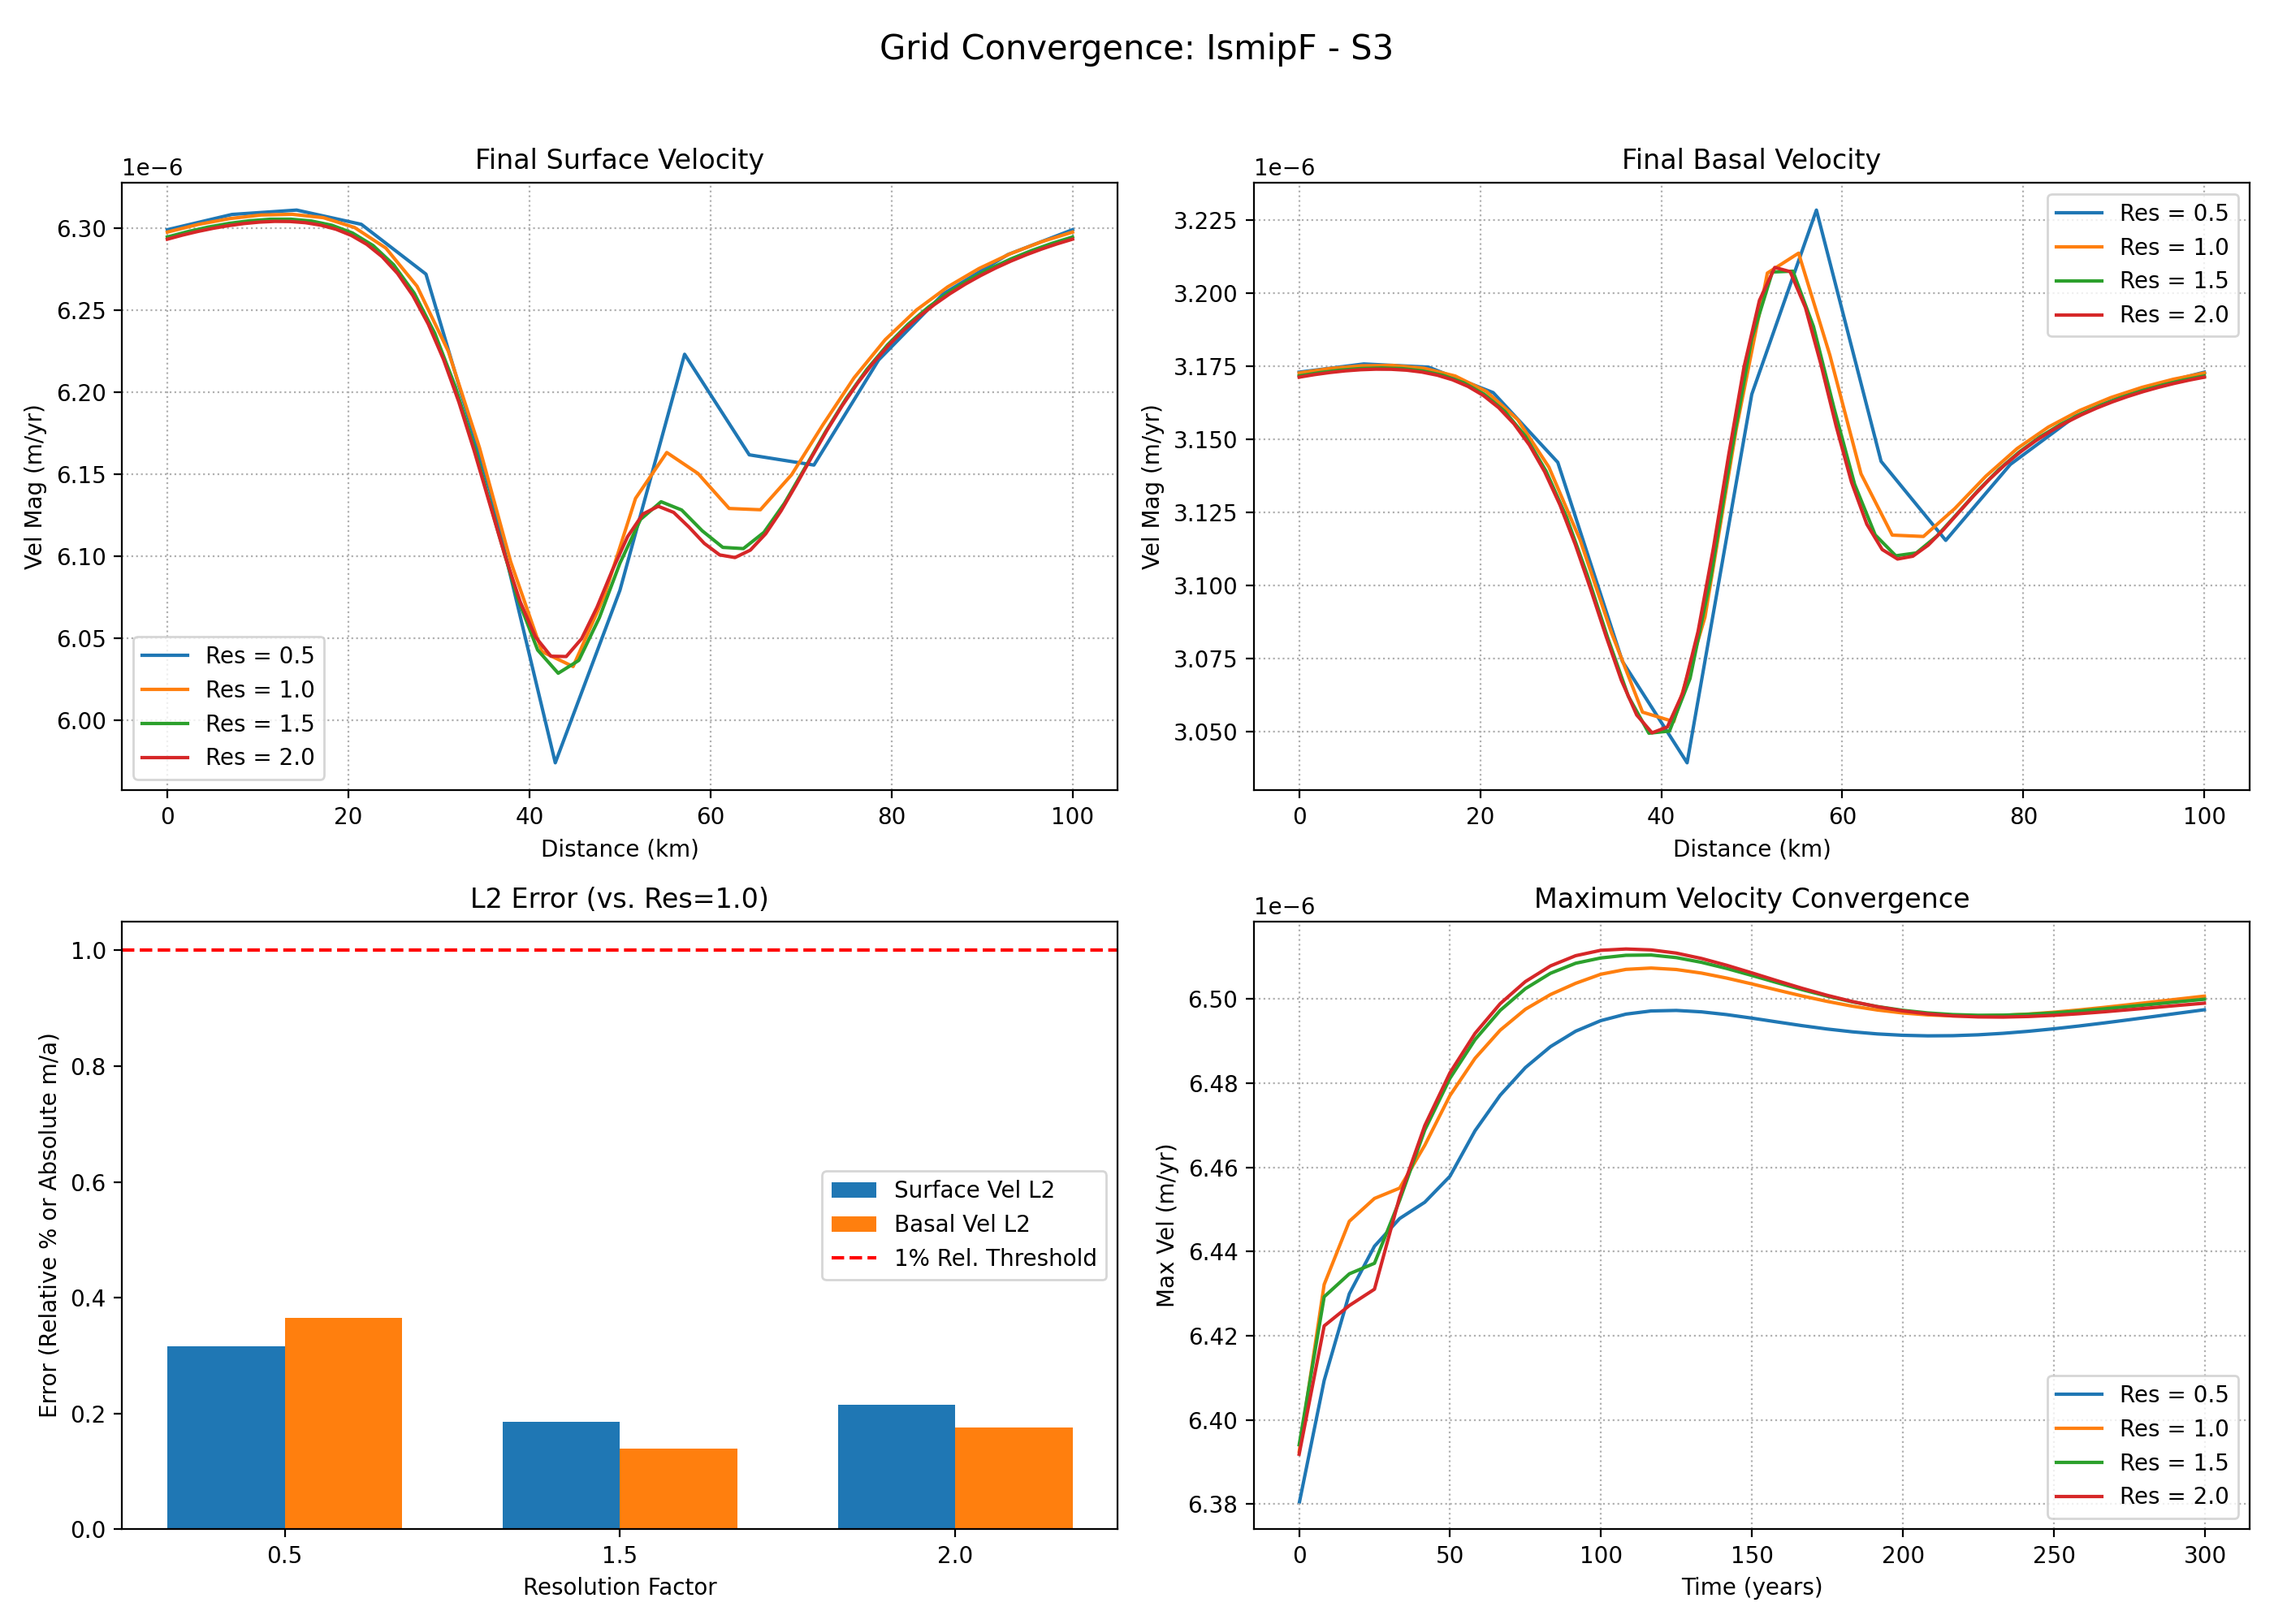
\includegraphics[scale=0.40]{figures/IsmipF_S3_convergence_summary.png}
    \caption{Grid convergence analysis for Scenario S3 (linear sliding, linear rheology, $n=1$). The four panels show: (top-left) final surface velocity profiles and (top-right) final basal velocity profiles for 16 different mesh resolutions; (bottom-left) the L2 relative error of each simulation compared to the highest-resolution mesh ($2.0\times2.0$), with a 1\% relative error threshold indicated by the dashed line; and (bottom-right) the evolution of the maximum velocity over the 300-year simulation period}
    \label{fig:grid_conv_S3}
\end{figure}
\begin{figure}[H]
    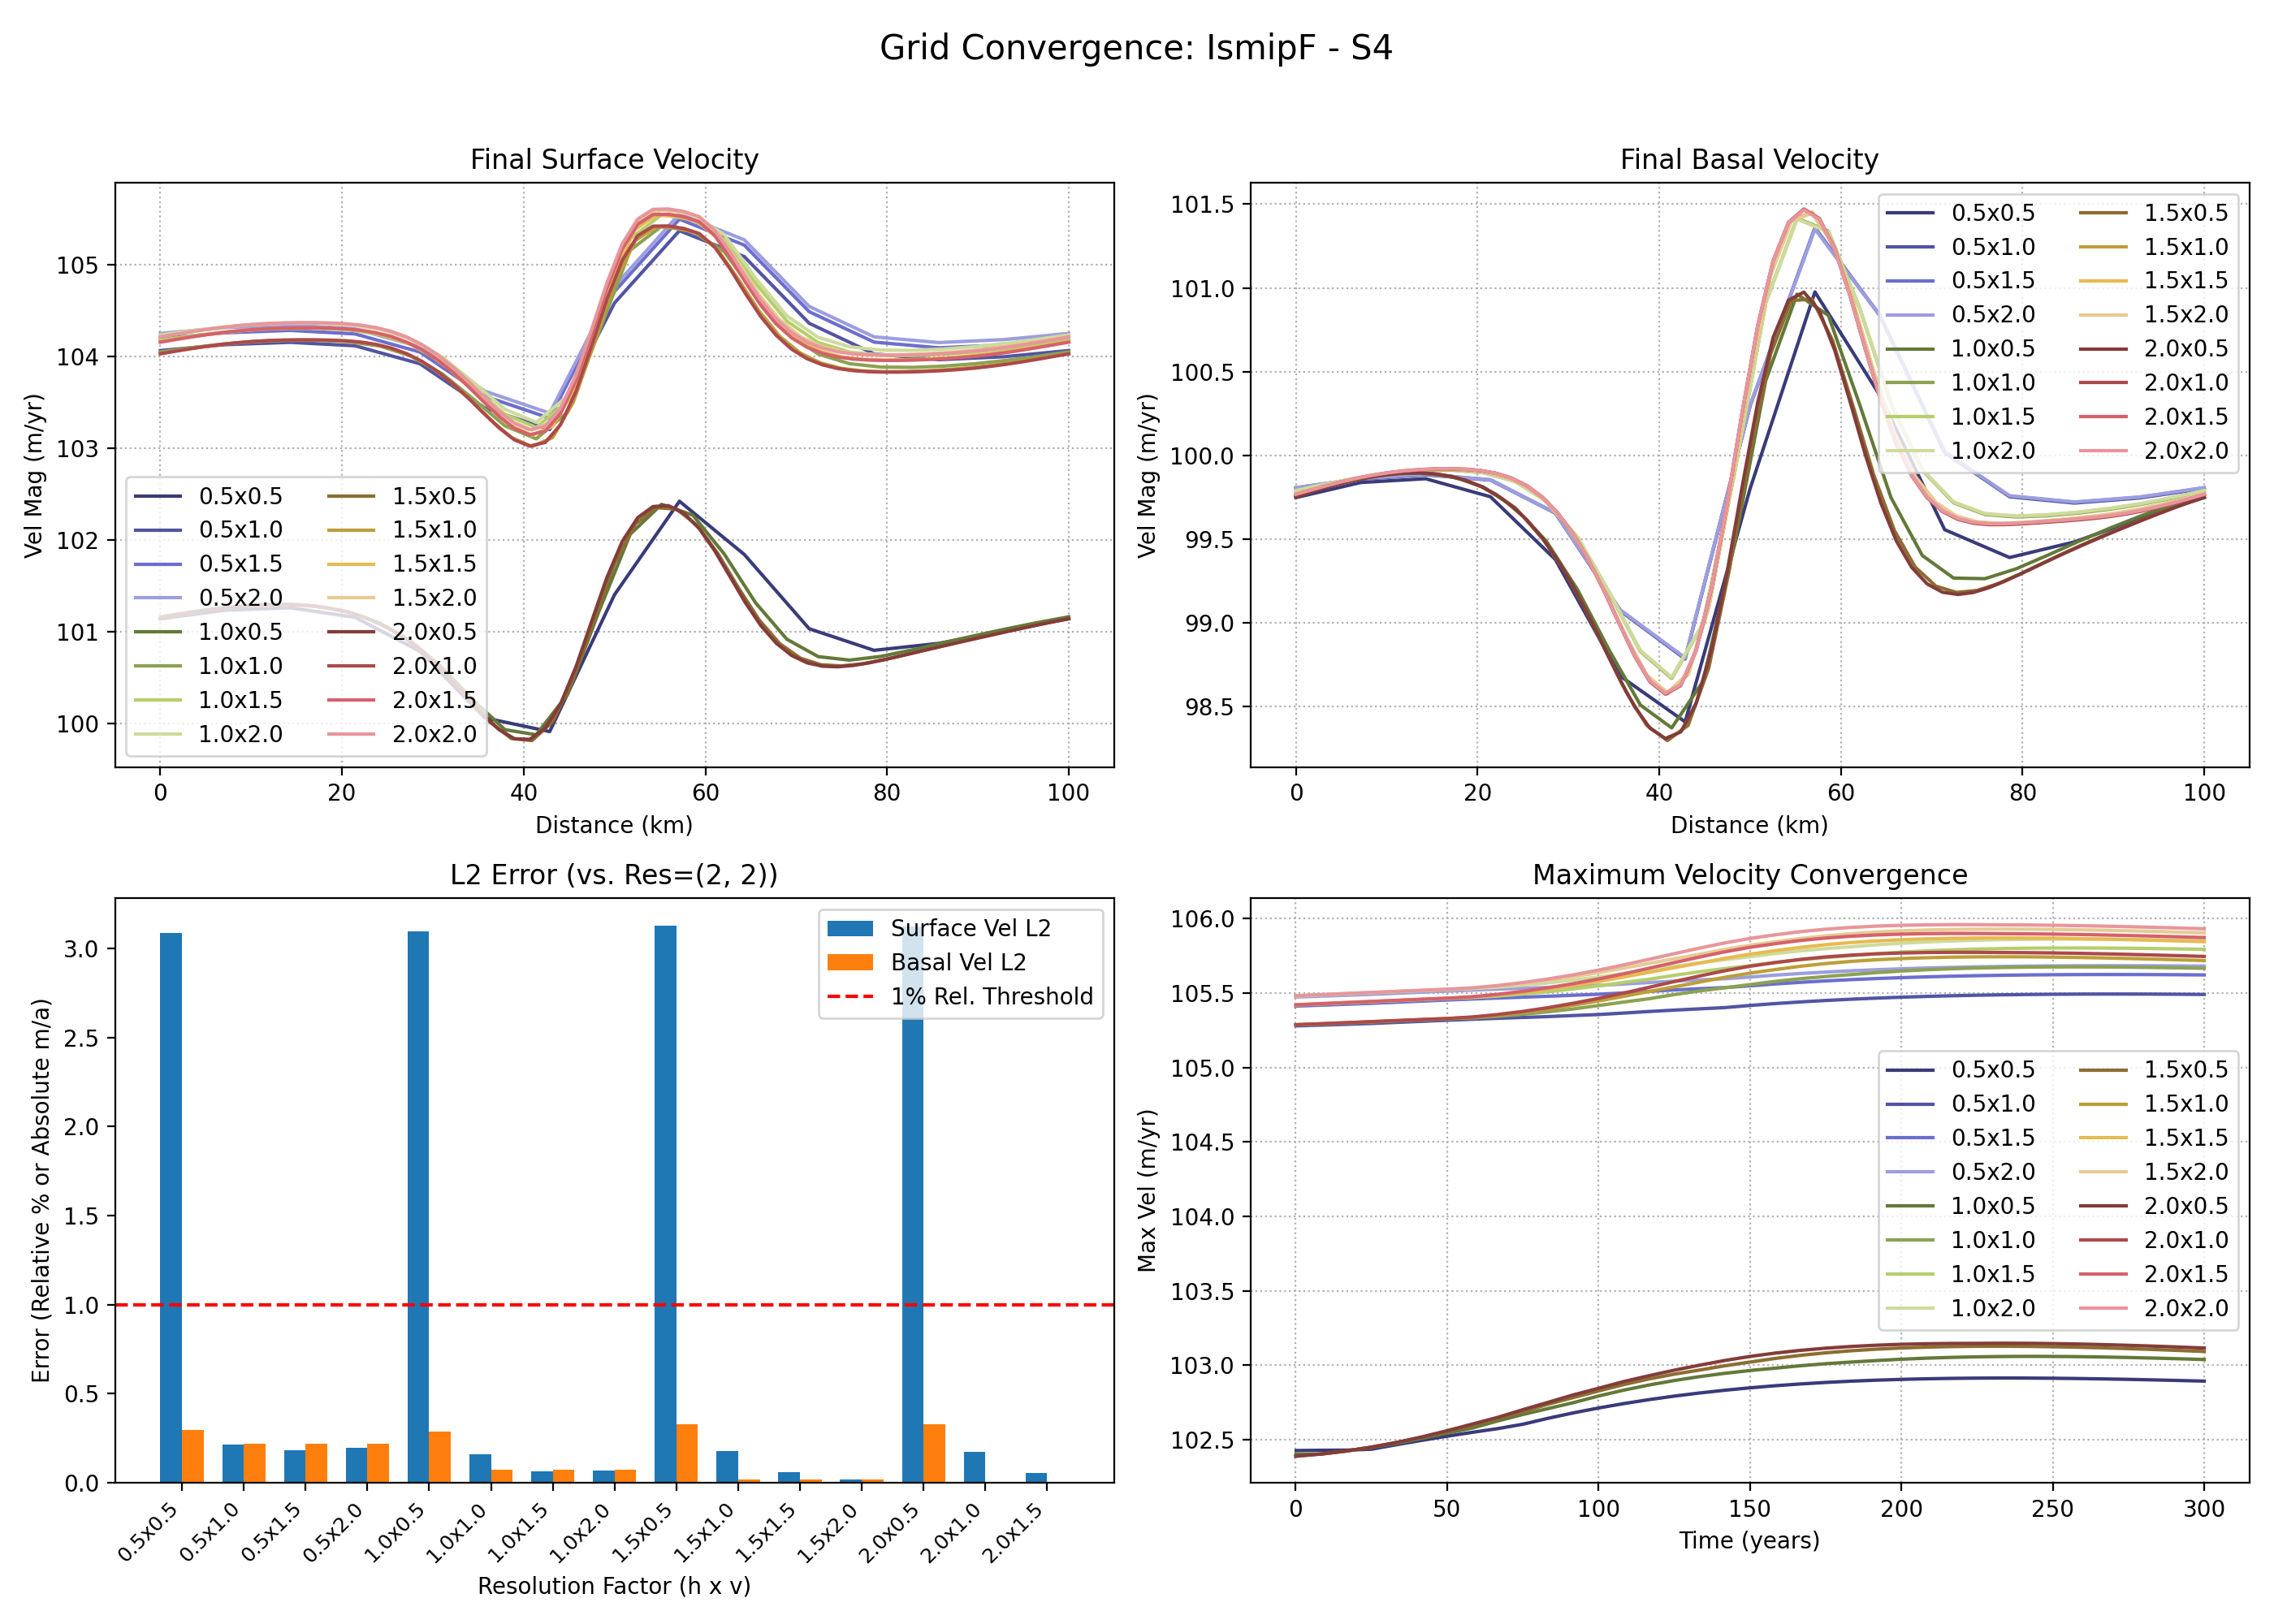
\includegraphics[scale=0.40]{figures/IsmipF_S4_convergence_summary.png}
    \caption{Grid convergence analysis for Scenario S4 (linear sliding, non-linear rheology, $n=4$). Another extension of ISMIP-HOM Experiment F. The convergence analysis demonstrates that non-linear scenarios exhibit high sensitivity to vertical resolution refinement, with low-resolution simulations showing the highest errors (with the relative error threshold only being achieved for simulations using the highest vertical resolution factor (2.0)) and converging to a slower flow state ($\approx~103$ m/a) compared to high-resolution runs ($\approx~106$ m/a).}
    \label{fig:grid_conv_S4}
\end{figure}
The primary metric of this script is the L2 relative error, a global, scale-dependent measure that quantifies the overall difference between two solutions. In my analysis, I chose a convergence threshold of $1\%$—since estimates of other uncertainties are expected to be larger than grid errors—when comparing the solutions to the baseline. If the L2 norm of the data is very close to zero (less than $10^{-6}$), the analysis reports the absolute error to avoid division by a tiny, unstable number. Otherwise, it calculates and reports the standard relative error as a percentage.

Convergence analyses show the simulations as most sensitive to vertical resolution. Particularly, non-linear rheology scenarios, where refining vertical resolution produces qualitatively different results. The convergence threshold of 1\% is only achieved for both S2 and S4 in Figure~\ref{fig:grid_conv_S4} with the finest resolution. This high sensitivity underscores the necessity of using converged, high-resolution simulations to generate the training data for BedSAT, ensuring the machine learning model is not learning artefacts from unresolved model physics.

The next phase of my research involves a suite of realistic synthetic bedrock topographies—closely mimicking the conditions found in Antarctica—in order to further inform the development of BedSAT.
\wordcount{progress} words in this section.

% \chapter{Numerics}
\begin{Figure}
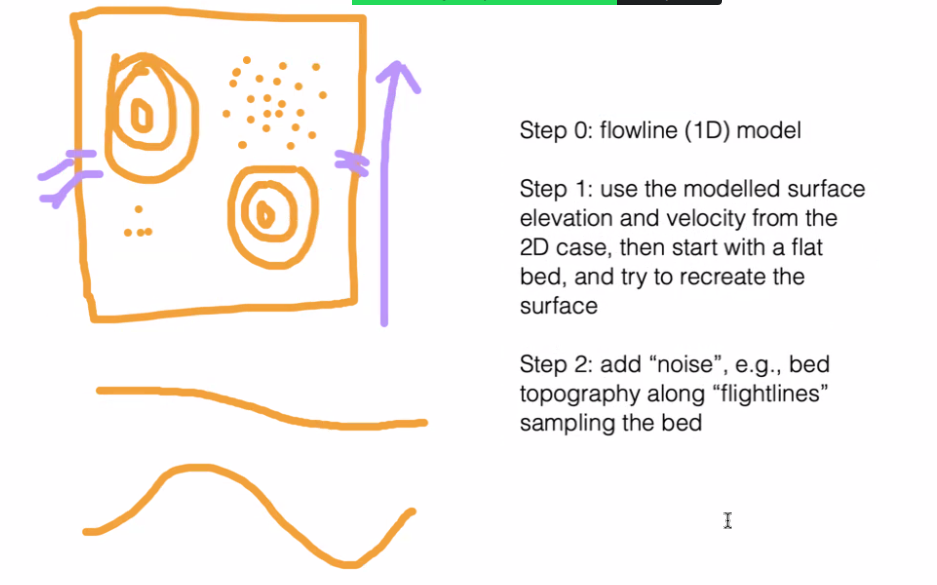
\includegraphics[width=0.9\linewidth]{steps.png}
\captionof{figure}{TODO}
\label{fig:first_sims}
\end{Figure}

\begin{Figure}
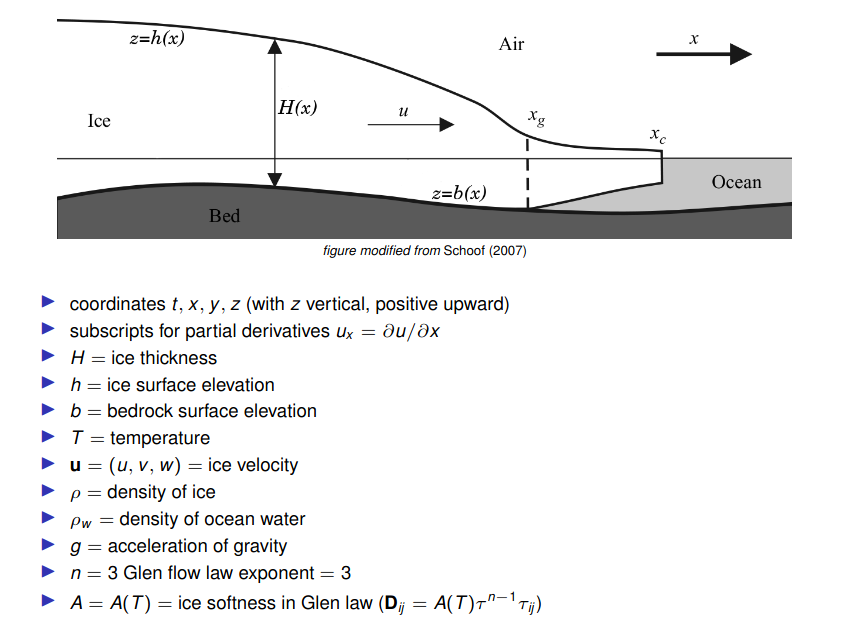
\includegraphics[width=0.9\linewidth]{numerical_modelling_of_glaciers.png}
\captionof{figure}{figure taken from\cite{modelling_ppt}}
\label{fig:parameters}
\end{Figure}

\section{ISSM: Continental-Scale Ice Sheet Modelling}
The Ice Sheet System Model (ISSM) was developed and is used for simulating ice sheet flow at continental scales. ISSM, a finite element, thermomechanical model, incorporates high-order stresses and high spatial resolution capabilities\cite{ISSM}. The Larour et al. (2012) ISSM paper discusses the different ice flow models within the software, including the full-Stokes, Blatter-Pattyn, Shallow-Shelf, and Shallow Ice Approximations, highlighting their individual strengths and limitations. It also explores numerical methods employed, such as static adaptive mesh refinement and inverse methods for parameter estimation. Finally, the study showcases the application of ISSM to the Greenland Ice Sheet, demonstrating its capacity to model the ice flow velocity with high accuracy, using data assimilation techniques to infer the basal drag coefficient.


% Study Guide
% Glossary of Key Terms

%     Shallow Ice Approximation (SIA): A simplified ice flow model that considers only vertical shear stresses and neglects horizontal stress gradients. Suitable for slow-moving ice in the interior of ice sheets.
%     Shallow Shelf Approximation (SSA): A simplified ice flow model that neglects vertical shear stresses and assumes depth-independent horizontal velocity. Appropriate for modeling floating ice shelves and fast-flowing ice streams.
%     Blatter-Pattyn Approximation (BP): A higher-order ice flow model that incorporates longitudinal stresses, making it suitable for simulating fast-flowing ice streams and regions with significant vertical shear.
%     Full-Stokes (FS): The most comprehensive and computationally expensive ice flow model, accounting for all stress components. Essential for accurately simulating ice flow near grounding lines.
%     Ice Sheet System Model (ISSM): A finite element, thermomechanical ice flow model that incorporates SIA, SSA, BP, and FS formulations to simulate ice sheet behaviour at various complexities and spatial resolutions.
%     Finite Element Method (FEM): A numerical method for solving partial differential equations by dividing the domain into smaller elements and approximating the solution within each element.
%     Adaptive Mesh Refinement: A technique used to refine the mesh in regions of high variability or complexity, enhancing model accuracy and efficiency.
%     Data Assimilation: The process of incorporating observational data into a model to improve its accuracy and predictive capabilities.
%     Basal Drag Coefficient: A parameter representing the frictional resistance between the ice sheet base and the underlying bedrock.
%     Grounding Line: The boundary where the ice sheet transitions from grounded ice to floating ice (ice shelf).
%     Calving: The process by which icebergs break off from the edge of a glacier or ice sheet.
%     InSAR: Interferometric Synthetic Aperture Radar, a remote sensing technique used to measure ice surface velocity.

% Quiz

% Instructions: Answer the following questions in 2-3 sentences.

%     What are the limitations of the Shallow Ice Approximation (SIA) and Shallow Shelf Approximation (SSA) in ice sheet modelling?
%     Why is the Full-Stokes (FS) model considered the most accurate representation of ice flow, and what makes its application challenging?
%     How does the Ice Sheet System Model (ISSM) integrate different ice flow approximations?
%     What is the importance of anisotropic adaptive mesh refinement in ISSM?
%     Describe the role of data assimilation in improving the accuracy of ice sheet models.
%     Why is the basal drag coefficient a crucial parameter in ice flow modeling?
%     Explain the concept of grounding line dynamics and its significance.
%     What is the process of calving, and why is it relevant to ice sheet mass balance?
%     How does ISSM handle the thermal regime of ice sheets?
%     What are some key challenges and future directions in ice sheet modeling using ISSM?

% Quiz Answer Key

%     SIA neglects horizontal stress gradients and is unsuitable for fast flow, while SSA ignores vertical shear, limiting accuracy near grounding lines.
%     FS accounts for all stress components, making it highly accurate, but its computational expense poses a challenge for large-scale applications.
%     ISSM offers SIA, SSA, BP, and FS formulations, allowing for different levels of complexity and computational efficiency.
%     It concentrates elements in dynamic regions like fast-flowing outlets, optimizing computational resources while preserving accuracy.
%     Data assimilation incorporates observations (e.g., surface velocity) to constrain model parameters and improve realism.
%     It governs basal friction, a key factor influencing ice flow velocity and the response to changes in temperature or basal conditions.
%     Grounding line dynamics refer to the movement of the grounding line, impacting ice discharge and contributing to sea level rise.
%     Calving is the breaking off of icebergs, a major process of mass loss from ice sheets, influencing their size and contribution to sea level.
%     ISSM includes a thermal model with heat conduction, advection, and a penalty scheme to ensure the temperature stays below the pressure melting point.
%     Challenges include improving grounding line dynamics, incorporating calving laws, and increasing spatial resolution, requiring more efficient numerical techniques and computational power.

% Essay Questions

%     Compare and contrast the four ice flow approximations (SIA, SSA, BP, and FS) implemented in ISSM, discussing their strengths, limitations, and appropriate applications.
%     Explain the process of data assimilation in ISSM, focusing on the inversion for the basal drag coefficient. Discuss the challenges and benefits of this approach.
%     Discuss the importance of accurate representation of grounding line dynamics in ice sheet models. What are the limitations of the current implementation in ISSM, and how can they be addressed in future development?
%     Describe the role of calving in ice sheet mass balance, and discuss the need to incorporate realistic calving laws in ice sheet models like ISSM.
%     Evaluate the potential of ISSM as a tool for projecting ice sheet contribution to future sea level rise. What are the key uncertainties and areas where the model can be improved?
% \wordcount{numerics} words in this section.
\begin{landscape}
\section*{Project timeline}
    \vspace{1cm}\hspace{-2.5em}
    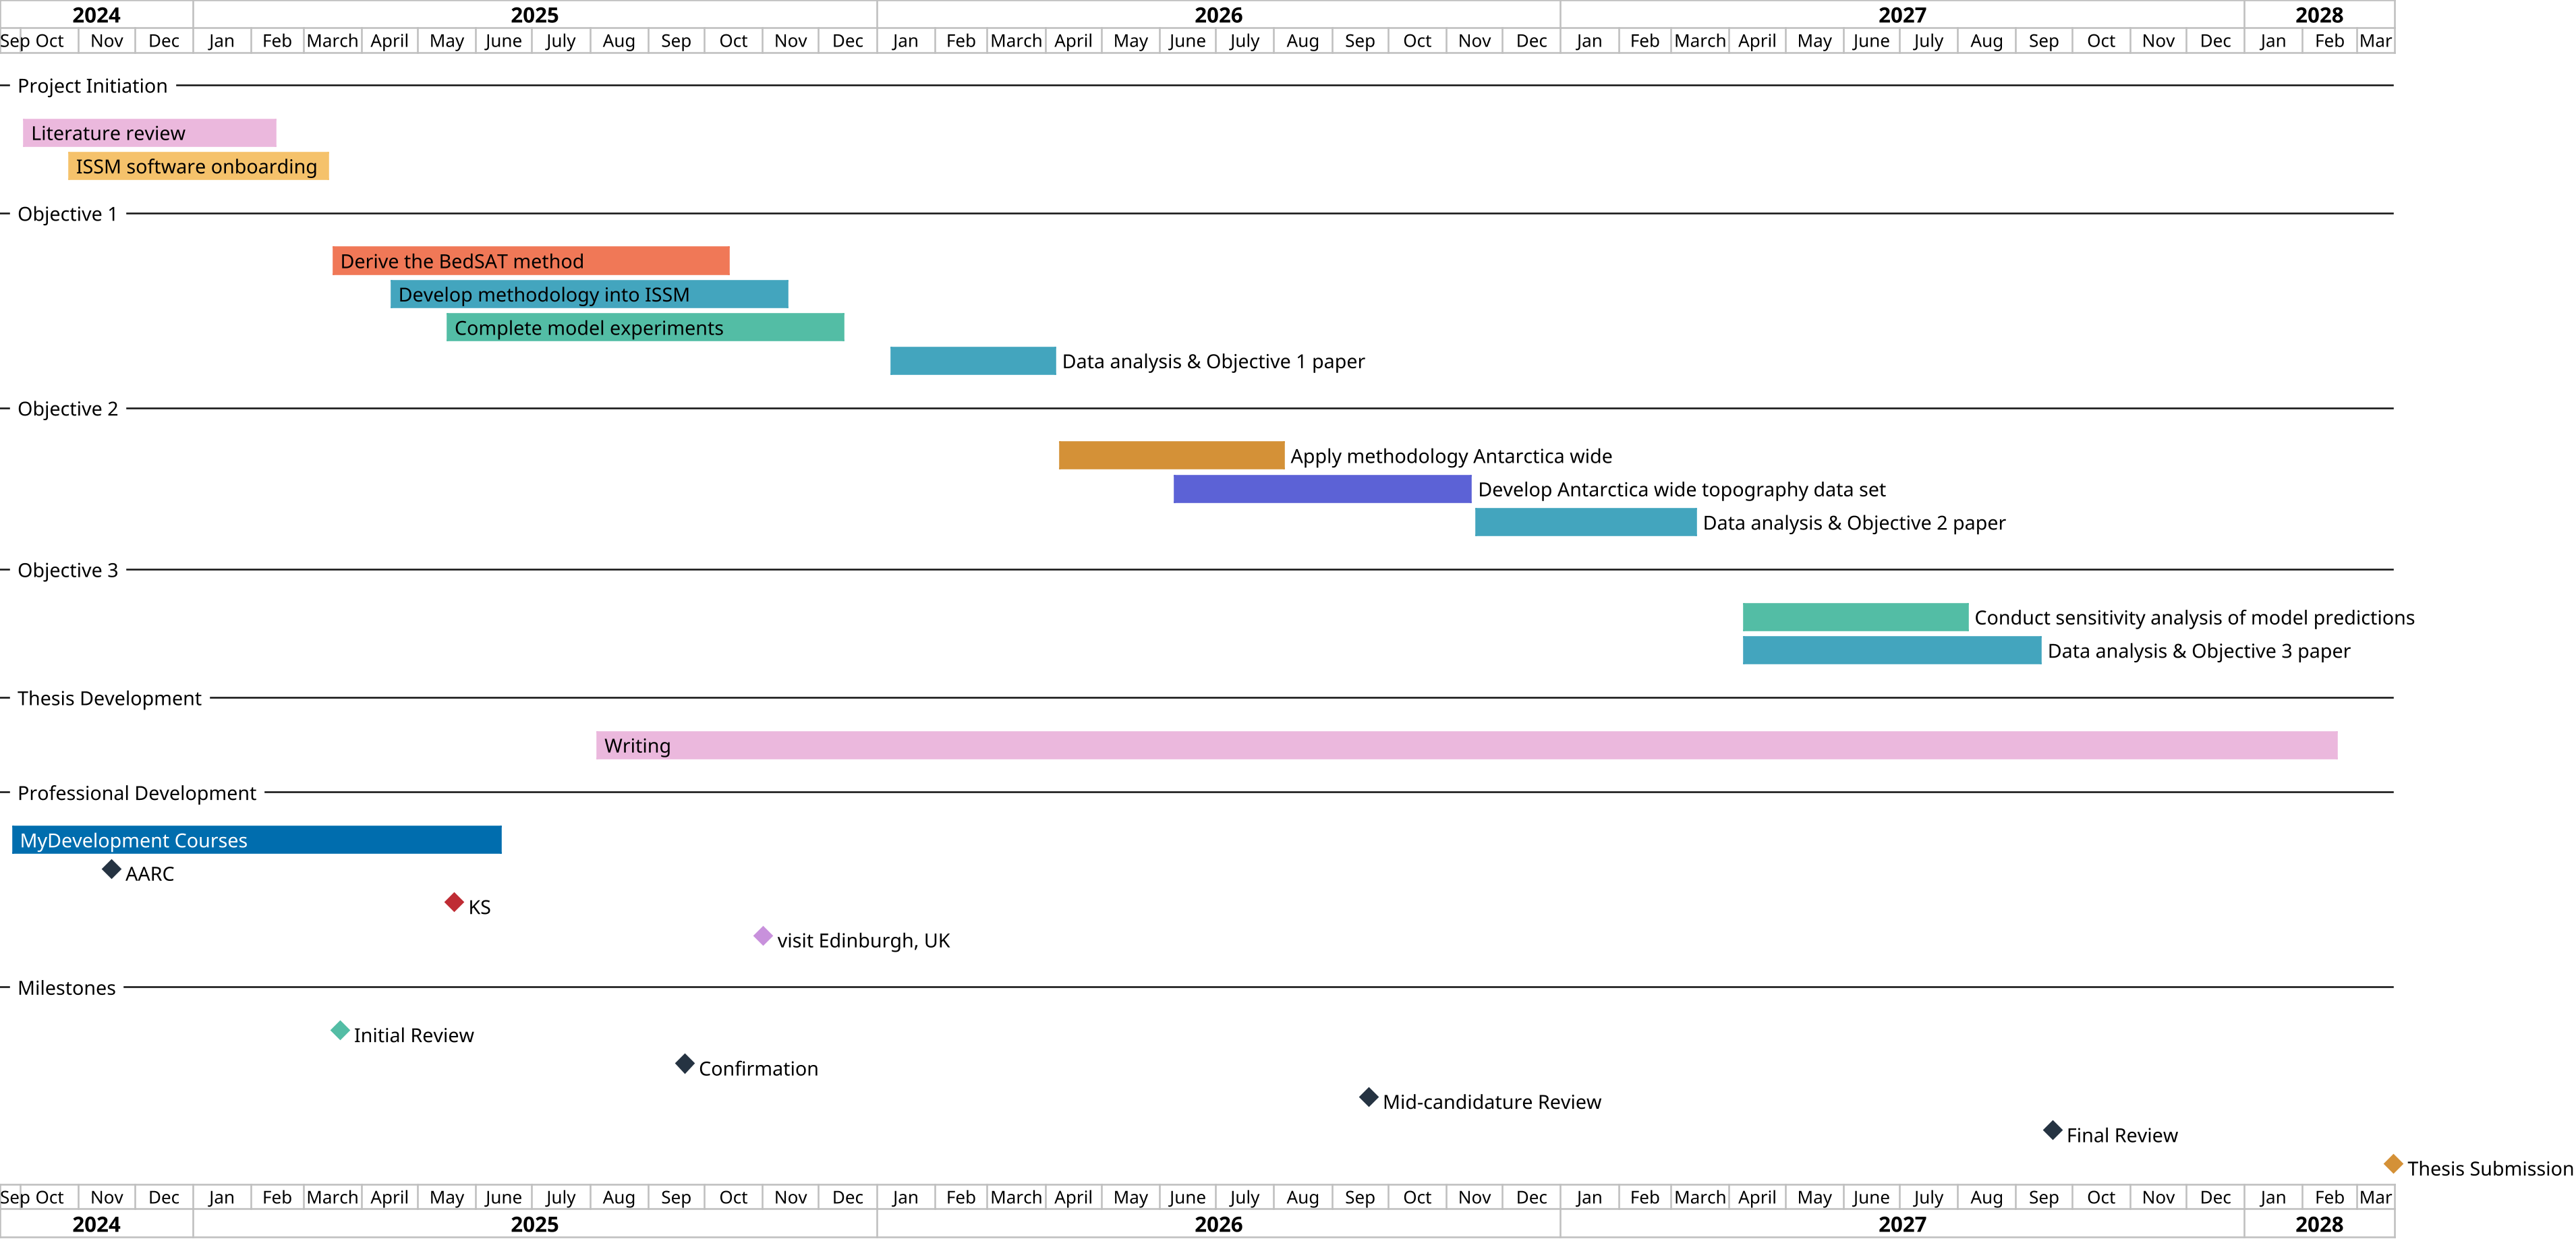
\includegraphics[width=0.85\linewidth]{timeline.png}
\end{landscape}

% \include{dynamics}
% % \wordcount{dynamics} words in this section.
% %
% \include{Conclusion}
% % \wordcount{Conclusion} words in this section.
% %
\chapter{Glossary of Key Terms}\label{glossary}
\begin{enumerate}
\item \textbf{Adaptive Mesh Refinement}: A technique used to refine the mesh in regions of high variability or complexity, enhancing model accuracy and efficiency.
\item \textbf{Asperity}: A protrusion or bump on a surface. Roughness The unevenness of a surface, characterized by the size and distribution of asperities.
\item \textbf{Basal Drag Coefficient}: A parameter representing the frictional resistance between the ice sheet base and the underlying bedrock.
\item \textbf{Basal Melt Rates}: The rate at which the underside of a glacier or ice sheet melts due to contact with warmer ocean water.
\item \textbf{Basal sliding}: Sliding occurring at the base of a glacier.
\item \textbf{Bed Topography}: The shape and elevation of the bedrock underlying a glacier or ice sheet.
\item \textbf{Bedrock Topography}: The shape and elevation of the solid rock surface beneath a glacier or ice sheet.
\item \textbf{Blatter-Pattyn Approximation (BP)}: A higher-order ice flow model that incorporates longitudinal stresses, making it suitable for simulating fast-flowing ice streams and regions with significant vertical shear.
\item \textbf{Calving}: The process by which icebergs break off from the edge of a glacier or ice sheet.
\item \textbf{Coefficient of sliding friction ($\mu$)}: The ratio of the shear stress to the normal stress during steady-state sliding.
\item \textbf{Coefficient of static friction ($\mu_s$)}: The ratio of the limiting static shear stress to the normal stress, indicating the resistance to sliding from rest.
\item \textbf{Data Assimilation}: The process of incorporating observational data into a model to improve its accuracy and predictive capabilities.
\item \textbf{Finite Element Method (FEM)}: A numerical method for solving partial differential equations by dividing the domain into smaller elements and approximating the solution within each element.
\item \textbf{Fourier Transform}: A mathematical tool used to decompose a signal, such as surface elevation data, into its constituent frequencies. This allows for analysis of specific spatial scales and features.
\item \textbf{Full-Stokes (FS)}: The most comprehensive and computationally expensive ice flow model, accounting for all stress components. Essential for accurately simulating ice flow near grounding lines.
\item \textbf{Global Mean Sea-Level Rise (SLR)}: The average increase in sea level across the globe due to various factors, including melting of glaciers and ice sheets, and thermal expansion of ocean water.
\item \textbf{Grounding Line}: The boundary where the ice sheet transitions from grounded ice to floating ice (ice shelf).
\item \textbf{Ice-Penetrating Radar}: A remote sensing technique used to map the bedrock topography beneath glaciers and ice sheets by transmitting radar waves through the ice.
\item \textbf{Ice Sheet System Model (ISSM)}: A finite element, thermomechanical ice flow model that incorporates SIA, SSA, BP, and FS formulations to simulate ice sheet behaviour at various complexities and spatial resolutions.
\item \textbf{InSAR}: Interferometric Synthetic Aperture Radar, a remote sensing technique used to measure ice surface velocity.
\item \textbf{Inversion}: A mathematical technique used to infer unknown parameters, such as bed topography, from observations of other variables, such as surface elevation and velocity.
\item \textbf{Limiting dynamic shear stress ($T_m$)}: The shear stress at which a glacier or ice block transitions from steady-state sliding to accelerated sliding.
\item \textbf{Kriging}: A geostatistical interpolation method that estimates unknown values at specific points by calculating weighted averages of known values from surrounding points, while accounting for spatial correlation and providing uncertainty estimates.
\item \textbf{Limiting static shear stress ($T_S$)}: The minimum shear stress required to initiate sliding from a resting position.
\item \textbf{Linear Perturbation Analysis}: A technique that examines the response of a system to small perturbations in its parameters, assuming a linear relationship between the perturbation and the response.
\item \textbf{Marine Ice Sheet Instability (MISI)}: A process where the grounding line of an ice sheet retreats into deeper water, leading to accelerated ice discharge and potentially unstoppable collapse.
\item \textbf{Momentum Balance}: The fundamental physical principle describing how forces control ice motion, expressed through the Navier-Stokes equations. In ice sheet modeling, it accounts for the balance between internal stresses, gravitational driving forces, and resistive forces (including drag at the bed and lateral margins).
\item \textbf{Normal stress ($N$)}: The force acting perpendicular to a surface, per unit area. In the context of glaciers, it is primarily the weight of the overlying ice.
\item \textbf{Null Space}: The set of all possible solutions to an inverse problem that do not contribute to the observed data. In the case of the work of \ref{Ockenden_2022}, features aligned with ice flow fall within the null space and cannot be resolved by the inversion.
\item \textbf{Pinning Point}: A topographic feature, such as a ridge or mountain, that can slow or temporarily halt the retreat of a glacier's grounding line.
\item \textbf{Regelation}: The process of melting under pressure and refreezing at lower pressure, potentially contributing to ice sliding.
\item \textbf{Retrograde Bedrock Slope}: A bedrock slope that deepens inland, making the ice sheet more susceptible to marine ice sheet instability.
\item \textbf{Rheology}: The study of how materials deform and flow under stress. In glaciology, it refers to the flow properties of ice.
\item \textbf{Shallow Ice Approximation (SIA)}: A simplified ice flow model that considers only vertical shear stresses and neglects horizontal stress gradients. Suitable for slow-moving ice in the interior of ice sheets.
\item \textbf{Shallow Shelf Approximation (SSA)}: A simplified ice flow model that neglects vertical shear stresses and assumes depth-independent horizontal velocity. Appropriate for modelling floating ice shelves and fast-flowing ice streams.
\item \textbf{Shallow-Ice-Stream Approximation}: A simplification of the ice flow equations that assumes the ice thickness is much smaller than the horizontal extent of the glacier, allowing for analytical solutions.
\item \textbf{Shear stress ($T$)}: The force acting parallel to a surface, per unit area. In the context of glaciers, it is the force driving glacier motion.
\item \textbf{Sliding}: The movement of a glacier over its bed by sliding rather than internal deformation.
\item \textbf{Slipperiness}: A measure of the ease with which ice can slide over its bed. It encompasses the influence of basal conditions like geology, hydrology, and sediment characteristics.
\item \textbf{Steady-state}: A condition where the glacier's flow and properties are constant over time, assuming a balance between ice accumulation and loss.
\item \textbf{Steady-state velocity ($V_b$)}: The constant velocity reached by a glacier or ice block when the driving shear stress is balanced by resisting forces.
\item \textbf{Stress Balance}: The equilibrium between the forces acting on an ice sheet, including gravity, basal friction, and internal ice stresses.
\item \textbf{Temperate ice}: Ice at or near its pressure-melting point.
\item \textbf{Transfer Functions}: Mathematical equations that describe the relationship between perturbations in bed properties and the resulting changes in surface variables.
\item \textbf{Volume Above Floatation (VAF)}: The volume of an ice sheet that is grounded on bedrock and contributes to sea-level rise if it melts or slides into the ocean.
\item \textbf{Wavelet Decomposition}: A mathematical technique that analyzes a signal by decomposing it into different frequency components at various spatial scales.
\end{enumerate}
% \include{appendix}
% % \wordcount{appendix} words in this section.

\bibliographystyle{unsrturl_mod}
\bibliography{mybib}
\end{document}


